\SourcePage{669}{674}
\section{Extraction of double-logarithmic terms in the vertex operator}

Corrections of the form $(\alpha L)^n$ (where $L$ is a large logarithm) can become appreciable, as noted at the end of \S~133, only at fantastically high energies and are therefore of theoretical interest alone. Amplitudes of actual scattering processes, however, also contain much larger corrections, of the form $(\alpha L^2)^n$. Terms having two powers of a logarithm for every power of $\alpha$ are called double-logarithmic terms.

The characteristic expansion parameter for double-logarithmic corrections is
\begin{equation}
\frac{\alpha}{\pi}\ln^2\frac{\varepsilon^2}{m^2};
\tag{135.1}
\end{equation}
here $\varepsilon$ denotes an energy occurring in the problem (for example, the total energy of the colliding particles in their center-of-mass frame). Perturbation theory is applicable only if this quantity is small; this condition fails at energies
\begin{equation}
\varepsilon\sim m\exp\left(\frac{1}{2}\sqrt{\frac{\pi}{\alpha}}\right)\sim3\cdot10^4m.
\tag{135.2}
\end{equation}

\SourcePage{670}{675}
Our aim will be to dispense with this restriction and obtain formulas valid under the condition
\begin{equation}
\frac{\alpha}{\pi}\ln^2\frac{\varepsilon^2}{m^2}\lesssim1.
\tag{135.3}
\end{equation}
This plainly requires summing the infinite series of corrections of every order $(\alpha L^2)^n$.

Double-logarithmic corrections occur in two classes of situations. The first comprises scattering processes through a fixed finite angle; as we saw in the preceding section, their cross sections always decrease in the high-energy asymptotic region. Here the double-logarithmic corrections are closely connected with infrared divergence. One example is elastic electron scattering by an external Coulomb field, whose first double-logarithmic correction to the cross section was found in \S~122. This section and the next are devoted to determining these corrections completely subject to (135.3).

The second class comprises reaction cross sections that decrease with increasing energy when the square of the momentum transfer is fixed, that is, at angles asymptotically tending to zero or to $\pi$. As shown in the preceding section, this behavior occurs in processes whose diagrams cannot be cut in the $t$- or $u$-channel across internal photon lines. In this case the double-logarithmic corrections are unrelated to infrared divergence. Backward electron--muon scattering, for which $u=\mathrm{const}$, will be considered as an example in \S~137.

We first observe that under condition (135.3) the single-logarithmic corrections satisfy
\[
\sim\frac{\alpha}{\pi}\ln\frac{\varepsilon^2}{m^2}\lesssim\sqrt{\frac{\alpha}{\pi}}\ll1
\]
and may therefore be omitted. Since $G$ and $D$ have no double-logarithmic corrections at all, these functions may now simply be replaced by their unperturbed values $G$ and $D$.

The calculation of the vertex operator $\Gamma$, by contrast, requires the summation of double-logarithmic terms generated by an infinite series of diagrams. That problem is addressed in the next section. We shall first describe a method for extracting the double-logarithmic terms from individual Feynman integrals before actually performing the integrations over all their variables (V.~V.~Sudakov, 1956).

Consider the first-order (in $\alpha$) correction to the vertex operator represented by diagram (117.1). Relabeling the variables, it is convenient to draw it here as

\SourcePage{671}{676}
\begin{equation}
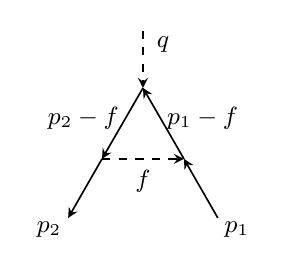
\begin{tikzpicture}[baseline=-.45ex,x=1cm,y=1cm,>=stealth,line width=.6pt,font=\small]
  \coordinate (t) at (0,1.05);
  \coordinate (l) at (-.52,.15);
  \coordinate (r) at (.52,.15);
  \draw[dashed,->] (0,1.78)--(t);
  \draw[->] (t)--(l);
  \draw[->] (l)--(-.95,-.60);
  \draw[<-] (t)--(r);
  \draw[<-] (r)--(.95,-.60);
  \draw[dashed,->] (l)--(r);
  \node[right] at (.05,1.60) {$q$};
  \node[left] at (-.18,.66) {$p_2-f$};
  \node[right] at (.18,.66) {$p_1-f$};
  \node[below] at (0,.13) {$f$};
  \node[below left] at (-.91,-.52) {$p_2$};
  \node[below right] at (.91,-.52) {$p_1$};
\end{tikzpicture}
\tag{135.4}
\end{equation}
or, analytically,
\begin{equation}
\begin{aligned}
\Gamma^{\mu(1)}(p_2,p_1;q)&={}\\
&=-\frac{ie^2}{4\pi^3}\int
\frac{\gamma^\nu(\gamma p_2-\gamma f+m)\gamma^\mu(\gamma p_1-\gamma f+m)\gamma_\nu\,d^4f}
{[(p_2-f)^2-m^2-i0][(p_1-f)^2-m^2+i0][f^2+i0]}.
\end{aligned}
\tag{135.5}
\end{equation}
We shall assume that
\begin{equation}
|q^2|\gg p_1^2,\ p_2^2,\ m^2,
\tag{135.6}
\end{equation}
where the legs $p_1$ and $p_2$ may be either physical or virtual. It follows from (135.6) that
\begin{equation}
|(p_1p_2)|\approx\frac12|q^2|\gg p_1^2,\ p_2^2,\ m^2,
\tag{135.7}
\end{equation}
so that the 4-vectors $p_1$ and $p_2$ have large components while their squares are small, a situation made possible by the pseudo-Euclidean character of the four-dimensional metric. Double-logarithmic terms arise precisely under conditions (135.6).

We shall see below that, in the integration over $d^4f$, comparatively small values of $f$ are important. Thus $f$ may be neglected in the numerator of the integrand, after which $\Gamma^{(1)}$ becomes
\begin{equation}
\Gamma^{\mu(1)}=-\frac{ie^2}{4\pi^3}\gamma^\nu(\gamma p_2+m)\gamma^\mu(\gamma p_1+m)\gamma_\nu I_1,
\tag{135.8}
\end{equation}
where
\begin{equation}
I_1=\int\frac{d^4f}{[(p_2-f)^2-m^2+i0][(p_1-f)^2-m^2+i0][f^2+i0]}.
\tag{135.9}
\end{equation}
The matrix factor in (135.8) can be simplified by noting that, in the diagrams where $\Gamma$ occurs, it is in effect always multiplied by the matrices $(\gamma p_2+m)$ and $(\gamma p_1+m)$:
\begin{equation}
(\gamma p_2+m)\Gamma(\gamma p_1+m).
\tag{135.10}
\end{equation}
Indeed, for virtual lines $p_1$ and $p_2$ these factors come from $G(p_1)$ and $G(p_2)$; for lines corresponding to real

\SourcePage{672}{677}
electrons, $\Gamma$ is multiplied by $\bar u_2$ and $u_1$, and the Dirac equations give
\[
\bar u_2=\bar u_2\frac{\gamma p_2+m}{2m},\qquad
u_1=\frac{\gamma p_1+m}{2m}u_1.
\]
Reordering the matrix factors and, at each step, using (135.7) to neglect the resulting squares $p_1^2$, $p_2^2$, and $m^2$ in comparison with $(p_1p_2)$, we obtain
\[
(\gamma p_2+m)\Gamma^{\mu(1)}(\gamma p_1+m)
\approx-\frac{ie^2}{\pi^3}(p_1p_2)(\gamma p_2+m)\gamma^\mu(\gamma p_1+m)I_1.
\]
Consequently, $\Gamma^{(1)}$ can finally be written as
\begin{equation}
\Gamma^{\mu(1)}=\frac{ie^2}{2\pi^3}\gamma^\mu tI_1,
\tag{135.11}
\end{equation}
where
\begin{equation}
t=q^2\approx-2(p_1p_2).
\tag{135.12}
\end{equation}
Notice that the integral $I_1$ converges at large $f$ and therefore needs no regularization.

The essential step in the calculation that follows is to introduce new, more convenient integration variables.

Resolve $f$ into components tangent and normal to the plane of $p_1$ and $p_2$:
\begin{equation}
f=up_1+vp_2+f_\perp\equiv f_\parallel+f_\perp,
\tag{135.13}
\end{equation}
\begin{equation}
f_\perp p_1=f_\perp p_2=0.
\tag{135.14}
\end{equation}
As the new variables we choose the coefficients $u$, $v$, and the quantity
\begin{equation}
\rho=-f_\perp^2.
\tag{135.15}
\end{equation}
Conditions (135.7) show that the metric in the $p_1p_2$ plane is pseudo-Euclidean. The time axis can consequently be chosen within this plane, making $f_\perp$ a spacelike 4-vector and hence $\rho>0$.

Temporarily denote by the indices $0$, $x$ the components of 4-vectors in the $p_1p_2$ plane, and by $y$, $z$ their components in the normal plane. To transform the 4-volume element $d^4f=d^2f_\perp d^2f_\parallel$ to the new variables, write
\[
d^2f_\perp=|f_\perp|d|f_\perp|d\varphi=\frac12d\rho\,d\varphi\to\pi d\rho
\]
(the integrand in (135.9) being independent of the angle $\varphi$). Furthermore,
\[
d^2f_\parallel=\left|\frac{\partial(f_0,f_x)}{\partial(u,v)}\right|du\,dv
=|p_{10}p_{2x}-p_{20}p_{1x}|du\,dv\approx\frac12|q^2|du\,dv.
\]

\SourcePage{673}{678}
Indeed, since the square $p_2^2$ is small, $p_{2x}^2\approx p_{20}^2$, and therefore
\[
(p_{10}p_{2x}-p_{20}p_{1x})^2\approx(p_{10}p_{20}-p_{2x}p_{1x})^2=(p_1p_2)^2=(q^2/2)^2.
\]
Thus
\begin{equation}
d^4f=\frac12|t|du\,dv\,d^2f_\perp\to\frac\pi2|t|du\,dv\,d\rho.
\tag{135.16}
\end{equation}
The subsequent calculation depends on the relation among $p_1^2$, $p_2^2$, and $m^2$. We consider two cases.

\textbf{Virtual electron lines.} Let the momenta $p_1$ and $p_2$ correspond to virtual electrons and satisfy
\begin{equation}
|p_1^2|,\ |p_2^2|\gg m^2.
\tag{135.17}
\end{equation}
We shall see that in this case the principal integration region producing the double-logarithmic expression is specified by
\begin{equation}
0<\rho\ll|tu|,\ |tv|;\qquad
\left|\frac{p_1^2}{t}\right|\ll|v|\ll1;\qquad
\left|\frac{p_2^2}{t}\right|\ll|u|\ll1.
\tag{135.18}
\end{equation}
Accordingly, in the denominator of the integrand in (135.9), $m^2$, $p_1^2$, $p_2^2$, and $f^2$ may be neglected compared with $(p_1f)$ or $(p_2f)$, giving
\begin{equation}
I_1=\int\frac{d^4f}{2(p_2f)\cdot2(p_1f)(f^2+i0)}.
\tag{135.19}
\end{equation}
For $(p_1f)$, $(p_2f)$, and $f^2$ we have
\[
\begin{aligned}
f^2&=(up_1+vp_2)^2-\rho\approx-tuv-\rho,\\
2(p_1f)&=2p_1(up_1+vp_2)\approx-tv,\\
2(p_2f)&\approx-tu.
\end{aligned}
\]
It follows that
\begin{equation}
I_1=-\frac{\pi}{2|t|}\int\frac{d\rho}{\rho+tuv-i0}\frac{du}{u}\frac{dv}{v}.
\tag{135.20}
\end{equation}
Under conditions (135.18), the $\rho$ integration extends from 0 to the smaller of $|tv|$ and $|tu|$, and yields
\begin{equation}
\int_0^{\min\{|tu|,|tv|\}}\frac{d\rho}{\rho+tuv-i0}
=\ln\min\left\{\frac1{|u|},\frac1{|v|}\right\}
+\begin{cases}i\pi,&tuv<0,\\0,&tuv>0.\end{cases}
\tag{135.21}
\end{equation}

\SourcePage{674}{679}
The logarithmic integration over $v$ is carried out from $-1$ to $-|p_1^2/t|$ and from $|p_1^2/t|$ to 1, and similarly for $u$. When (135.21) is substituted in (135.20), the $du\,dv$ integral of the first term vanishes because its integrand is odd. For the second term, the integration runs over intervals where $u$ and $v$ have the same sign if $t<0$, and opposite signs if $t>0$. In either case the regions $v>0$ and $v<0$ make equal contributions after the integration over $u$. We thereby find (the sign of the integral is the sign of $t$)
\begin{equation}
I_1=\frac{i\pi^2}{2t}\cdot2
\int_{|p_2^2/t|}^1\frac{du}{u}
\int_{|p_1^2/t|}^1\frac{dv}{v}
=\frac{i\pi^2}{t}\ln\left|\frac{t}{p_1^2}\right|\ln\left|\frac{t}{p_2^2}\right|.
\tag{135.22}
\end{equation}
Finally, substituting $I_1$ into (135.11), we obtain
\begin{equation}
\Gamma^{\mu(1)}(p_2,p_1;q)=-\frac{\alpha}{2\pi}\gamma^\mu
\ln\left|\frac{q^2}{p_1^2}\right|\ln\left|\frac{q^2}{p_2^2}\right|,
\tag{135.23}
\end{equation}
\[
|q^2|\gg|p_1^2|,\ |p_2^2|\gg m^2.
\]

\textbf{Physical electron legs.} Now let the momenta $p_1$ and $p_2$ correspond to real electrons, so that
\begin{equation}
p_1^2=p_2^2=m^2.
\tag{135.24}
\end{equation}
The relevant integration region is then
\begin{equation}
0<\rho\ll|tu|,\ |tv|;\qquad 0<|v|,\ |u|\ll1.
\tag{135.25}
\end{equation}
Since $p_1^2-m^2=p_2^2-m^2=0$, neglecting $p_1^2$ and $p_2^2$ compared with $(p_1f)$ or $(p_2f)$ again reduces the integral (135.9) to the form (135.19). To remove the infrared divergence that now appears, however, a finite photon mass $\lambda\ll m$ must also be introduced in the photon propagator (cf.\ \S~117):
\begin{equation}
I_1=\int\frac{d^4f}{2(p_1f)\cdot2(p_2f)(f^2-\lambda^2+i0)}.
\tag{135.26}
\end{equation}
We next have
\[
f^2\approx-tuv-\rho,\qquad
2(p_1f)\approx-tv+2m^2u,\qquad
2(p_2f)\approx-tu+2m^2v,
\]
and hence
\begin{equation}
I_1=-\frac{\pi}{2|t|}\int
\frac{d\rho}{\rho+tuv+\lambda^2-i0}\,
\frac{du}{u-\tau v}\,\frac{dv}{v-\tau u},
\qquad \tau=\frac{2m^2}{t}\ll1.
\tag{135.27}
\end{equation}

\SourcePage{675}{680}
After the $\rho$ integration, carried out as in (135.21), we find
\[
I_1=-\frac{i\pi^2}{2|t|}\iint\frac{du}{u-\tau v}\frac{dv}{v-\tau u},
\]
where the integration is subject to $tuv+\lambda^2<0$. The regions $v>0$ and $v<0$ once again give equal contributions, and integration over $u$ gives
\begin{equation}
\begin{aligned}
I_1&=\frac{i\pi^2}{t}\int_0^1dv\int_{\delta/v}^1
\frac{du}{(u-\tau v)(v-\tau u)}\\
&=\frac{i\pi^2}{t}\int_0^1
\ln\left|\frac{\tau\delta-v^2}{(\delta-\tau v^2)(\tau-v)}\right|\frac{dv}{v},
\end{aligned}
\tag{135.28}
\end{equation}
where $\delta=\lambda^2/|t|$, $|\delta|\ll|\tau|$, and $|\tau|\ll1$ has been used.

In the integral (135.28), three regions of $v$ give double-logarithmic expressions:
\[
\mathrm{I})\ |\tau|\ll v\ll1,\qquad
\mathrm{II})\ \sqrt{\delta/\tau}\ll v\ll|\tau|,\qquad
\mathrm{III})\ \sqrt{\tau\delta}\ll v\ll\sqrt{\delta/\tau}.
\]
(For definiteness we suppose that $\sqrt{\delta/\tau}\ll|\tau|$. The result does not depend on this assumption.) Making the appropriate approximations in each region, we obtain
\begin{equation}
I_1=\frac{i\pi^2}{2t}\left(\ln^2\frac{|t|}{m^2}+4\ln\frac{|t|}{m^2}\ln\frac{m}{\lambda}\right).
\tag{135.29}
\end{equation}
Finally, substitution in (135.11) gives
\begin{equation}
\Gamma^{\mu(1)}(p_2,p_1;q)=-\frac{\alpha}{4\pi}\gamma^\mu
\left(\ln^2\frac{|q^2|}{m^2}+4\ln\frac{|q^2|}{m^2}\ln\frac{m}{\lambda}\right),
\tag{135.30}
\end{equation}
\[
|q^2|\gg|p_1^2|=|p_2^2|=m^2,
\]
in agreement with (117.21).
